\section{Constraint Mapping}
\label{sec:mapper}

Let $\mathcal{S}$ denote the sentences passed to the mapper, either all preprocessed sentences or the subset retained by the classifier. For each $s_i \in \mathcal{S}$, the mapper returns a denial constraint (DC) $\varphi_i = \neg(p_1 \land \cdots \land p_\ell)$ over the dataset schema, or no output if $s_i$ does not express a constraint or cannot be linked to the schema.

Recall from Section~\ref{sec:problem} that DC predicates can take several forms, including comparisons between an attribute and a constant (e.g., \texttt{t.A = c}), between two attributes of the same tuple (e.g., \texttt{t.A > t.B}), or between attributes across tuples (e.g., \texttt{t1.A = t2.A}), as well as null checks and membership tests over permitted values.
The mapping task is therefore to interpret a sentence, identify the relevant schema elements, select the predicates on those elements that capture the constraint intuition, and produce an executable \emph{violation condition}. In this sense, it is related to Text-to-SQL~\cite{yu2018spider}, as both tasks aim to connect a natural language segment to schema-aware logical expressions. One key difference is that Text-to-SQL typically retrieves satisfying records, whereas our target is a conjunction of predicates that identify a constraint violation.

\begin{example}[Mapping to DC predicates]
\label{ex:mapping}
Consider the sentence ``A score of 0--13 results in a grade of A'' from the NYC restaurant inspection regulations. This sentence states that scores in the range 0--13 must be associated with grade A. The corresponding violation condition is:
\[
\texttt{t.score} \geq \texttt{0} \land \texttt{t.score} \leq \texttt{13} \land \texttt{t.grade} \neq \texttt{`A'}
\]
Any tuple satisfying all three predicates violates the rule. \qed
\end{example}

Mapping regulatory text to DCs is challenging because the same rule may be expressed in many different ways, often with implicit references to schema elements, literals, or tuple relationships. \altic{[R2-O2, R2-O3, R1-O5, R3-O2] PONTO CRÍTICO (queixa dos 3 revisores). Adicionar uma subseção dedicada de ``novidade metodológica'' articulando a contribuição ALÉM dos prompts. Tese de defesa: o cerne não são os prompts, mas (a) o espaço de predicados controlado derivado do schema que impede colunas alucinadas/operadores não suportados, (b) a forma de violação (não-satisfação) como alvo, e (c) os checks pós-construção/orphan-predicate sobre os dados. Fazer uma tabela explícita delimitando, componente a componente, o que é ADAPTADO de Text-to-SQL (schema linking, decomposição em estágios, como RESDSQL e DIN-SQL) vs. o que é NOVO (espaço de predicados como vocabulário controlado, forma de violação, grounding por orphan-predicate). Sem isso, paper é lido como ``engenharia de prompt''.}
We therefore rely on LLM-based mappers, motivated by their strong performance on related semantic parsing tasks such as Text-to-SQL~\cite{llmTEXT2SQLSurvey2025}. However, unrestricted LLM generation is unreliable in our setting, it is known that LLMs  can hallucinate column names and use unsupported operators~\cite{dail2025,llmTEXT2SQLSurvey2025,DBLP:conf/dexa/DociniAO25}. 
We also observed that LLMs tend to output predicates describing valid states rather than violations, so we introduce hints toward violations in the prompt.

To make mapping tractable and reliable, our design follows two principles. First, we derive a \emph{predicate space} from the dataset schema and use it as a controlled vocabulary. The mapper must either select predicates from this space or instantiate typed placeholders within predefined predicate templates. This reduces the search space and prevents ill-formed outputs. Second, the mapper is biased toward \emph{precision}. Incorrect mapping can generate false violations and corrupt downstream checks, whereas an unmapped sentence can still be marked for manual inspection.

We implement three mapper variations that share the same predicate space but differ in how they use it. The \emph{single-prompt mapper} (Section~\ref{sec:mapper:llm}) and \emph{multi-step mapper} (Section~\ref{sec:mapper:multistep}) operate at the sentence level: the former performs the full mapping in a single LLM call, while the latter decomposes the task into focused LLM calls interleaved with deterministic checks. The \emph{document-level mapper} (Section~\ref{sec:mapper:document}) operates at the document level in a single LLM call, without native sentence-to-constraint traceability.


\subsection{Predicate Space}
\label{sec:mapper:predicate-space}

Traditional DC discovery operates over a \emph{predicate space}, that is, the set of predicates allowed to appear in candidate constraints~\cite{chu2013discovering,Pena2019DiscoveryDC}. Because discovery methods enumerate and validate combinations of predicates, this space is kept small, which limits expressiveness~\cite{chu2013discovering}.

Our setting requires a richer predicate space. Regulatory text frequently refers to explicit literals, enumerations, ranges, nullability conditions, and string formats that are not covered by traditional DC discovery spaces.\altic{[R3-O7] Corrigir a alegação: o revisor apontou (com razão) que DCs tradicionais JÁ cobrem null checks e comparação com literais/constantes. Restringir a frase ao que realmente falta no espaço clássico: ranges, enumerações (IN) e padrões de string (LIKE). Reescrever para ``...ranges, enumerations, and string formats not covered by traditional DC discovery spaces'', removendo ``explicit literals'' e ``nullability conditions'' da lista de ausências.} We therefore extend the predicate space with typed predicate templates that can be instantiated with literals extracted from text. Importantly, \system\ does not enumerate candidates DC  over this larger space. Instead, it uses the space as a controlled vocabulary for mapping, which avoids candidate explosion while preserving syntactic validity.

\smallskip\noindent\textbf{Predicate templates.}
We derive a finite set of predicates and predicate templates from the schema, while the data instance is used to support specific instantiations and validation steps. We consider the following categories:
\begin{enumerate}
    \item \textbf{Cross-tuple predicates} compare attributes across two tuples (e.g., \texttt{t1.A = t2.A}, \texttt{t1.A > t2.B}). We allow $\{=,\neq\}$ for type-compatible attributes and additionally $\{<,\leq,>,\geq\}$ for numeric attributes.
    \item \textbf{Same-tuple predicates} compare two attributes within one tuple (e.g., \texttt{t1.A $\leq$ t1.B}), capturing intra-tuple rules.
    \item \textbf{Null predicates} (\texttt{t1.A IS NULL}, \texttt{t1.A IS NOT NULL}) capture requiredness and conditional missingness constraints.
    \item \textbf{Attribute--constant predicates} compare an attribute to a constant $c$ (e.g., \texttt{t1.A = c}, \texttt{t1.A $\geq$ c}).
    \item \textbf{Pattern predicates} encode string-format and substring conditions (e.g., \texttt{t1.A LIKE p}).
    \item \textbf{Set predicates} encode membership in small enumerations (e.g., \texttt{t1.A IN C}).
    \item \textbf{Arithmetic predicates} compare an arithmetic expression over numeric attributes of the same tuple with an attribute or a constant (e.g., \texttt{t1.A $\geq$ c * t1.B}), when the schema enables arithmetic for those attributes.
\end{enumerate}
For categories 4--7, the mapper instantiates the placeholders $c$, $p$, or $C$ using literals extracted from the sentence.
\altic{[R2-O4] Adicionar (i) análise de COBERTURA destas 6 categorias contra o conjunto de gold constraints de cada dataset (quantas regras-alvo são expressáveis), e (ii) discussão explícita dos limites de expressividade, em particular a exclusão de agregações e aritmética temporal, que forçou derivar manualmente a coluna ``days-until-next-inspection'' no Restaurant. Assumir essa limitação como escopo, não escondê-la.}

\smallskip\noindent\textbf{Predicate restrictions.}
To avoid semantically uninformative or implausible predicates, we adopt a filtering principle from DC discovery~\cite{chu2013discovering}. Order predicates are generated only for numeric attributes. Cross-tuple and same-tuple predicates are generated only for type-compatible pairs and are further pruned using observed value overlap, helping eliminate comparisons between unrelated columns.
Nonetheless, our extensions with predicate templates, constants, patterns, and sets expand the predicate space from the dozens common in DC discovery to several hundred in some datasets. This space is impractical for traditional data profiling, where the enumeration cost grows exponentially with the number of predicates. In our approach, the larger predicate space remains practical because we use it only as a constrained target language for mapping, not as a search space for enumerating combinations.


\smallskip\noindent\textbf{Schema-driven, on-demand predicate space.}
Materializing the full space does not scale to wide schemas: with arithmetic and
code-set templates, the space of a 135-column table reaches hundreds of thousands
of templates, most of which are irrelevant to any given sentence. \system\
therefore stores only a \emph{schema description} and generates predicates on
demand. For each column, the description records its type, the comparison and
arithmetic operators it admits, its domain values when it has at most a few
distinct values, and a short natural-language description. Descriptions are
written once, offline, by an LLM from a deterministic profile of the data (type,
null rate, distinct values, ranges, frequent values, format patterns, and observed
code--label pairs); when an official data dictionary is available, its
definitions are merged into the description of the corresponding columns (we do
this for HMDAZ, using the FFIEC field definitions). At mapping time, once the
relevant columns of a sentence are selected, the predicates of the categories
above are generated only for those columns, under the same restrictions. For a
fixed instance and fixed options, the generated set equals the full space
restricted to the selected columns, so the controlled vocabulary is unchanged;
only its materialization is deferred.

\subsection{Single-Prompt Mapper}
\label{sec:mapper:llm}

The single-prompt mapper performs the full mapping in a single LLM call. 
We design the prompt around three elements: the schema and predicate space as a controlled vocabulary, a small set of examples covering the main constraint patterns, and predicate specifications to guide the model in understanding and mapping violation conditions. Given an input sentence, the model returns either a list of predicates drawn from the predicate space or \texttt{null}. 
Figure~\ref{fig:mapprompt} summarizes the prompt structure.
In the current version, the prompt is restricted to the columns retrieved for
the sentences of each batch (three sentences per call): columns are ranked by
the embedding similarity between the sentence and the column name and
description (semantic retrieval), and the prompt carries the description and
domain values of each retrieved column (column context) together with the
predicates generated for them. The model must also state, for each sentence,
the condition under which a tuple violates the rule (\texttt{violated\_when})
before writing the DC, which makes the violation form explicit. Rules that
reference unknown columns or compare a column with a constant of the wrong type
are returned to the model once, with the error message.





\begin{figure}[!ht]
\centering
\footnotesize
\begin{tabularx}{\linewidth}{p{0.2\linewidth}X}
\toprule
\textbf{Definition} &
\hlc[neutralbg]{A denial constraint (DC) is a conjunction of predicates 
that \emph{cannot} all hold simultaneously in a dataset. DC predicates 
must encode \emph{violations} of data quality rules, not valid states.} \\
\midrule
\textbf{Violation Form} &
\hlc[neutralbg]{``must be X'' $\Rightarrow$ \texttt{!= X};
``must not be X'' $\Rightarrow$ \texttt{= X};} \\
\midrule
\textbf{Cross-Tuple} &
\hlc[neutralbg]{Signals such as ``same \ldots'', ``repeated'', or ``consecutive'' introduce \texttt{t1}, \texttt{t2}, and a join predicate on the shared key.} \\
\midrule
\textbf{Context} &
\hlc[contextbg]{Table schema + top-$k$ frequent values per column.} \newline
\hlc[contextbg]{List of possible predicates (predicate space).} \\
\midrule
\textbf{Examples} &
\hlc[yesbg]{``Value must be at least 100''}
$\Rightarrow$ \texttt{["t1.value < 100"]} \newline
\hlc[yesbg]{``Same ID must share status''}
$\Rightarrow$ \texttt{["t1.id = t2.id", "t1.status != t2.status"]} \newline
\hlc[nobg]{``The system performs well''}
$\Rightarrow$ \texttt{null} \\
\midrule
\textbf{Output} &
\hlc[neutralbg]{Array of length $n$, one entry per input sentence; \texttt{null} for non-constraints. Predicates must come from the predicate space.} \\
\bottomrule
\end{tabularx}
\caption{Prompt structure for the single-prompt mapper. Examples are 
representative, as the full prompt covers threshold, set-membership, 
field-comparison, null, cross-tuple, and non-constraint cases. The colors represent: 
\csquare{contextbg}\,Data context; \csquare{yesbg}\,constraint example; 
\csquare{nobg}\,non-constraint; \csquare{neutralbg}\, instructions.}
\label{fig:mapprompt}
\end{figure}

\smallskip\noindent\textbf{Violation form.}
Without explicit guidance, LLMs generally tend to output predicates describing 
\emph{satisfying} tuples rather than \emph{violating} ones. Since 
regulatory sentences typically describe what must hold, the mapper must 
find predicates expressing a violation condition---as in Example~\ref{ex:mapping}, 
where the correct output is \texttt{grade $\neq$ `A'}, not \texttt{grade $=$ `A'}. 
We make this criterion explicit in the prompt through a small set of examples.



\smallskip\noindent\textbf{Cross-tuple constraints.}
Some rules address relationships between records rather than conditions 
within a single record. In these cases, the mapper must introduce two 
tuple aliases and a join predicate on the shared identifier.%---producing, for instance, \texttt{t1.id = t2.id} alongside the distinguishing predicate. 
Including cues such as ``for the same'' in the prompt
already suffices for the model to generalize reliably to the variety of phrasings in which such predicates appear.
\altic{[R1-O8] Esclarecer o escopo das constraints cross-tuple: o revisor perguntou como condições que valem para todas/maioria das tuplas (estilo differential dependencies) são encontradas e validadas. Deixar explícito que o alvo são DCs com no máximo 2 variáveis de tupla, com semântica universal de violação (sem agregação/contagem sobre maioria), e que differential dependencies ficam fora do escopo. Se forem suportadas, explicar o mecanismo de validação.}


\smallskip\noindent\textbf{Literal grounding.}
Many constraints require grounding numeric thresholds, strings, or small 
enumerations. A recurring failure is to produce literals in the wrong 
format or casing. To mitigate this, we include in the prompt the top-$k$ 
frequent values per column as a domain context, which anchors 
literals to the dataset representation. In practice, we found that fewer than ten 
samples per column usually suffice for the model to capture the relevant patterns.

The mapper returns at most one DC per sentence. If the sentence is not mappable, it returns \texttt{null}. We parse the output and validate every predicate against the schema: it must reference existing columns, use operators admitted by their types, compare them with constants of the right type, and have no uninstantiated placeholders. Membership in the generated predicate space is not enforced for this mapper; we report it instead (out-of-space predicates). Malformed outputs are retried a fixed number of times, and invalid rules are returned once to the model with the error. If all attempts fail, the sentence produces no constraint. To prevent incorrect mappings from affecting downstream checks, we intentionally keep this stage conservative.


\smallskip\noindent\textbf{Batch processing.}
As in the classifier (Section~\ref{sec:classifier}), we support batch processing by concatenating multiple indexed sentences into one prompt and returning one output per index. 
%We use the same moderate batch sizes and fallback strategy.

\subsection{Multi-Step Mapper}
\label{sec:mapper:multistep}
The single-prompt mapper needs to parse several subtasks in one call: schema linking, predicate selection, literal linking, and  violation form. In this setting, errors in early steps might sometimes propagate. For example, a wrong column choice may break predicate selection, a hallucinated literal yields a syntactically valid but semantically meaningless constraint, and a non-constraint sentence triggers an unnecessary mapping attempt. Recent work in Text-to-SQL shows that decomposing semantic parsing into multiple stages, especially separating schema linking from later query building decisions, often improves accuracy~\cite{DBLP:conf/dexa/DociniAO25,redsql2025,dail2025,llmTEXT2SQLSurvey2025}. 

\altic{[R2-O5] Justificar POR QUE quatro estágios e adicionar ablação mais fina do que Single-vs-Multi: remover/reordenar estágios (p.ex. sem rule-filter, sem schema-linking separado, ordem trocada) para mostrar que o ganho vem da DECOMPOSIÇÃO e não apenas de mais chamadas ao LLM. Caso contrário o ganho do Multi-Step é atribuível a ``mais compute''.}
We propose a multi-step mapper that breaks down mapping into several LLM calls, with deterministic checks in between.
The process uses four LLM calls, where each call receives the output from the previous step. Sentences that cannot be mapped are
removed before constraint construction. After construction, data-driven checks
eliminate constraints that have incorrect literals.

Figure~\ref{fig:multistep-pipeline} illustrates the control flow of our multi-step mapper and
Figure~\ref{fig:multistepprompt} provides a summary of its prompts in each step.

%, andFigure~\ref{fig:multistep-trace} illustrates an execution trace.



\begin{figure}[ht!]
    \centering
    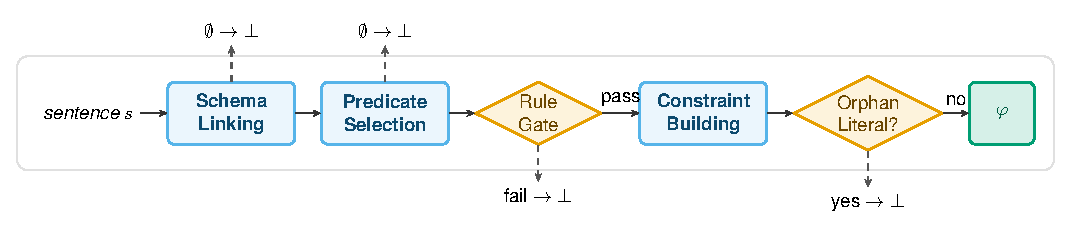
\includegraphics[width=\columnwidth]{diagramas/multistep_diagram.pdf}
    \caption{Multi-step mapper control flow.}
    \label{fig:multistep-pipeline}
\end{figure}



\begin{figure}[ht!]
\centering
\footnotesize
\begin{tabularx}{\linewidth}{p{0.13\linewidth}p{0.28\linewidth}X}
\toprule
\textbf{Step} & \textbf{Context} & \textbf{Task} \\
\midrule

\textbf{Schema} &
\hlc[contextbg]{Full schema, column profiles, predicate space} &
\hlc[neutralbg]{Identify all columns relevant to $s$: direct mentions, synonyms, and derived concepts.}
\hlc[nobg]{Abort if no concept maps to any column with defined predicates.} \\

\midrule

\textbf{Predicates} &
\hlc[contextbg]{$\hookrightarrow$ Columns from Schema step} \newline
\hlc[contextbg]{Predicate space restricted to those columns} \newline
\hlc[contextbg]{Column profiles} &
\hlc[neutralbg]{Select predicates and predicate templates from the restricted predicate space and identify the constraint pattern for $s$ (value mapping, temporal bound, functional dependency, required field, or conditional rule).}
\hlc[nobg]{Abort if no predicate or predicate template fits.} \\

\midrule

\textbf{Rule filter} &
\hlc[contextbg]{$\hookrightarrow$ Columns and predicates from Predicates step} &
\hlc[neutralbg]{Decide whether $s$ expresses a specific, data quality rule verifiable from column values alone.} \newline
\hlc[nobg]{Reject: process descriptions, permissions, vague quantifiers, physical conditions.} \newline
\hlc[yesbg]{Accept: value mappings, temporal bounds, functional dependencies, required fields, conditional rules.} \\

\midrule

\textbf{Construction} &
\hlc[contextbg]{$\hookrightarrow$ Predicates and predicate templates from Predicates step} \newline
\hlc[contextbg]{Column profiles} &
\hlc[neutralbg]{Substitute predicate placeholders with literals from $s$ and return the constraint in violation form: a conjunction of predicates that must not hold simultaneously.} \\

\bottomrule
\end{tabularx}
\caption{Prompt structure of the multi-step mapper. Context narrows progressively. The rule filter runs after predicate selection but before construction, avoiding unnecessary LLM calls on non-rules.
\csquare{contextbg}\,input context (variable per step);
\csquare{yesbg}\,accept signal;
\csquare{nobg}\,abort\,/\,reject signal;
\csquare{neutralbg}\,fixed instruction.}
\label{fig:multistepprompt}
\end{figure}

\smallskip\noindent\textbf{Schema linking.}
This step identifies the columns relevant to the sentence, including implicit 
references and derived concepts. We prompt the model to return the set of columns relevant for the sentence, since operating over a smaller, relevant subset reduces the risk of incorrect predicate selection in the later step. If no column with defined predicates can be aligned to any concept in the sentence, we reject the sentence for mapping.

\smallskip\noindent\textbf{Predicate selection.} The mapper uses only columns retained by schema linking. Given the column names, profiles, and restricted predicate spaces, it selects predicates and predicate templates (requiring literals) that together form the DC pattern. We separate column selection from predicate selection to address distinct subproblems: schema linking determines which attributes are relevant to a sentence, while predicate selection determines how those attributes are combined into a denial-constraint structure. This decomposition reduces the DC structural search space and helps avoid predicates that, while individually plausible, do not compose into a valid constraint. This design aligns with prior results in text-to-SQL, where having a dedicated structural parsing step has been shown to improve accuracy~\cite{resdsql2023}.

\smallskip\noindent\textbf{Rule filter.}
This step determines whether the sentence can be mapped to a DC under the schema-grounded interpretation obtained so far. Unlike the classifier in Section~\ref{sec:classifier}, the rule filter has access to the candidate columns and predicates selected for the sentence. This improves the semantic reliability of the decision, since many sentences that appear rule-like in isolation may fail to support a coherent executable constraint once their concepts are grounded in the schema and tied to candidate predicates. %We therefore place the filter after predicate selection, where this evidence is available. %, but before construction, to avoid unnecessary literal grounding for sentences that should still be rejected.
%
%\smallskip\noindent\textbf{Constraint building.}
%This step builds the final DC by instantiating the selected predicate templates with literals extracted from the sentence. Since the candidate columns and predicate forms have already been fixed, construction no longer needs to search the full predicate space. Instead, it resolves the value-level details required by the selected templates, such as numeric thresholds, categorical values, ranges, patterns, and small enumerations. We use the column profiles with sample values to align these literals with the dataset's representation. The goal is to preserve details such as casing, abbreviations, and formatting used in the data and map that to the term in the sentence.. 
%The output is produced as a set of predicates representing  in violation form. Restricting this step to grounded instances of previously selected templates reduces the risk of hallucinated predicates and ill-formed constraints~\cite{pourreza2023din,picard2021}.

\smallskip\noindent\textbf{Constraint building.}
This step instantiates the selected predicate templates with the literals needed to form the final DC. At this point, the candidate columns and predicate types have already been fixed, so the task is no longer to explore the full predicate space, but to realize a small set of grounded predicate instances. The model resolves value-level details such as numeric thresholds, categorical constants, intervals, string patterns, and short enumerations, and aligns them with the dataset representation using column profiles and sample values. This grounding is important because the text and the data often use different representations. A sentence may describe a concept in natural language, while the table records it as an abbreviation, code, or differently formatted value. The output is a set of predicates in violation form, which are then assembled into the final DC. Framing this stage as grounded instantiation rather than open-ended generation substantially narrows the construction problem and makes unsupported predicates and malformed expressions less likely~\cite{pourreza2023din,picard2021,lin-etal-2020-bridging}.


\smallskip\noindent\textbf{Post-construction checks.}
After constructing a candidate DC, both sentence-level mappers apply a set of validation checks to ensure that the generated constraints are both executable and semantically plausible. First, we verify the structural validity of the DC: each predicate must belong to the predicate space, reference valid schema columns, use type-compatible operators, and contain no uninstantiated placeholders. Next, we apply a data-based grounding check for unsupported literals. For each predicate with literals involving equality, string inequality, \texttt{LIKE}, or set membership, we issue an existence query against the dataset. If no tuple can satisfy the predicate, we refer to it as an \emph{orphan predicate}, i.e.,, a predicate that is syntactically valid but unsupported by the data instance. Any constraint containing a orphan predicate is disregard for validation, although it may be retained for documentation purposes. 
Numeric bounds and \texttt{null} predicates are excluded from this check because their validity is structural rather than value-based.
If parsing fails, the mapper retries a small fixed number of times; if all attempts fail, no constraint is returned.

%\begin{figure}[t]
%    \centering
%    \includegraphics[width=\columnwidth]{diagramas/multistep_diagram_trace.pdf}
%    \caption{Example execution trace of the multi-step mapper.}
%    \label{fig:multistep-trace}
%\end{figure}


\subsection{Document-level mapping}
\label{sec:mapper:document}

The mappers described above operate at sentence granularity, which is the primary focus of this work. As noted in Section~\ref{sec:problem}, the Text-to-Constraints problem admits other granularities: a segment may span multiple sentences, a paragraph, or an entire document, and a single segment may yield multiple constraints. We also integrate a document-level mapper into \system\ to study this alternative granularity. While sentence-level processing is the primary focus of this work, document-level mapping serves as a useful complementary mode, and a broader study of granularity choices and sentence-grouping strategies is left for future work.

This setting introduces additional challenges, as regulatory documents contain substantial amounts of text that are not directly related to data quality constraints, including headings, definitions, explanatory passages, and procedural descriptions.

The document-level mapper submits the entire document to the LLM in a single call and
returns a flat set of DCs, where the DC count is determined by the document
content rather than the number of input sentences. It reuses the predicate space,
violation-form instructions, and literal-grounding conventions developed for the
sentence-level mappers, so the controlled vocabulary and instructions carry over
without modification. 

The prompt used in this mode differs from the single-prompt mapper (Figure~\ref{fig:mapprompt}) primarily in the output format, replacing sentence-indexed predictions with an unordered list of constraints. As before, every returned predicate is validated against the predicate space and discarded if it references unknown columns, uses unsupported operators, or contains uninstantiated placeholders.




%\begin{algorithm}[ht!]
%\caption{Multi-Step Mapper}
%\label{alg:multistep}
%\small
%\begin{algorithmic}[1]
%\Input{sentence $s$, predicate space $\mathcal{P}$, dataset $\mathcal{D}$}
%\Output{denial constraint $\varphi$, or $\bot$}
%\State $C \gets \Call{SchemaLinking}{s, \mathcal{P}}$
%\State \textbf{abort if} $C = \emptyset$
%\State $P, \pi \gets \Call{PredicateSelection}{s, C, \mathcal{P}|_C}$
%\State \textbf{abort if} $P = \emptyset$
%\State \textbf{abort if} $\neg\Call{FilterNonRules}{s,C,P,\pi}$
%\State $\varphi \gets \Call{BuildConstraint}{s, C, P}$
%\State \textbf{abort if} $\varphi = \emptyset$
%\State \textbf{abort if} $\Call{DeadLiteral}{\varphi, \mathcal{D}}$
%\State $cnt \gets \Call{Execute}{\varphi, \mathcal{D}}$
%\State \Return $\varphi$ \textbf{if} $\Call{CheckViolations}{\varphi, cnt}$ \textbf{else} $\bot$
%\end{algorithmic}
%\end{algorithm}